\section{Diffusion models}\label{diffusion Models}

Diffusion models have emerged as a prominent method in generative modeling, offering distinct advantages over traditional models like Variational Autoencoders (VAEs) and Generative Adversarial Networks (GANs). Specifically addressing the limitations in data quality and generation efficiency that VAEs and GANs encounter, diffusion models present a novel approach. They operate by progressively perturbing data with noise and then learning to reverse this process, a methodology that enables the generation of highly realistic and diverse new samples.

~\cite{yangdiffusionSummary} distingueshe between three main approaches that dominate the study of diffusion models, which are going to be discussed shortly: Denoising Diffusion Probabilistic Models (DDPMs) \citep{hoDDPMs,sohlDDPM}, Score-based Generative Models (SGMs) \citep{song2019SGM}, and Stochastic Differential Equations (Score SDEs) \citep{song2020score, song2021maximum}. Each of these models has its own set of strengths and challenges, contributing uniquely to the development of Diffusion Models.

\subsection{Denoising Diffusion Probabilistic Models}

Central to the concept of Denoising Diffusion Probabilistic Models (DDPMs) are two Markov chains: the forward chain and the reverse chain, also known as the forward and reverse diffusion processes \citep{sohlDDPM}. These processes are illustrated in Figures~\ref{fig:figureForwardProcess} and~\ref{fig:figureReverseProcess}. 

The forward diffusion process, sharing some similarities with VAEs, focuses on a latent feature space of the initial data distribution. However, DDPMs differ in that the forward process in DDPMs ``is fixed to a Markov chain that gradually [over a span of T steps] adds Gaussian noise to the data according to a variance schedule \(\beta_1, \ldots, \beta_T \)''~\cite{hoDDPMs}. This process gradually pertubes the data's structure, eventually resulting in an image of pure noise, with the aim of gradually steering the data distribution towards a more manageable prior distribution \citep{yangdiffusionSummary, pooleDreamfusion}. 

The mathematical formulation of the forward process is given by \citeauthor{martinez2023understanding}:

\[
q(x_t | x_{t-1}) = \mathcal{N}(x_t; \sqrt{1 - \beta_t}x_{t-1}, \beta_t I) \quad \text{where} \quad \sqrt{1 - \beta_t}x_{t-1} = \mu_t \quad \text{and} \quad \beta_t I = \Sigma_t
\] 

In this equation, the model first adjusts the previous data point \( x_{t-1} \) to get \( x_t \), the data point at the current step. This adjustment follows a Gaussian distribution and is done using the term \( \sqrt{1 - \beta_t} x_{t-1} \), which slightly reduces the intensity or strength of the previous data point \citep{sohlDDPM, hoDDPMs}. This controlled approach helps maintain a balance between the original data and the noise, ensuring that the noise doesn't overwhelm the data too quickly. Once this preparatory step is completed, the model then introduces noise. The level of noise added at each step is determined by the parameter \( \beta_t \), where a higher value means more noise is added \citep{kingma2023variationalDM}. The way noise is added is described by the covariance matrix \( \beta_t I \), where \( I \) is the identity matrix \citep{croitoru2023diffusion}. This matrix ensures that noise is added to each element of the data in an independent and uniform manner, evenly distributing the noise across all parts of the data. The importance of this noise-adding process lies in its role in teaching the model the structure and characteristics of noise. By gradually adding noise to the data, the model learns how images degrade step by step, knowledge that is crucial for the reverse process of DDPMs.

The process of adding noise over the entire sequence from the original data point \( x_0 \) to \( x_T \) is captured another formular by \citeauthor{martinez2023understanding}:

\[q(x_{1:T} | x_0) = \prod_{t=1}^T q(x_t | x_{t-1}) \] 

Built upon the Markov property, the formula implies that each step depends solely on the previous step, allowing for a systematic and gradual transformation from \( x_0 \) to \( x_T \) \citep{martinez2023understanding}. This methodical approach provides a detailed understanding of the data's evolution at each noise addition stage, giving a complete view of the transition probabilities throughout the forward diffusion process.

\begin{figure}[ht]
\centering
  \includegraphics[width=1\columnwidth]{figures/manta_DDMP3.png}
  \caption{Illustration of the Forward Diffusion Process in DDPMs: This figure demonstrates the gradual addition of Gaussian noise to an image over multiple steps. Each subsequent image from left to right shows an increased level of noise, culminating in the far-right image, which represents a state of pure noise.}\label{fig:figureForwardProcess}
\end{figure}

The reverse diffusion process, illustrated in Figure~\ref{fig:figureReverseProcess}, employs a neural network parameterized by \(\Theta\) to approximate the inverse of the forward process \citep{sohlDDPM, yangdiffusionSummary}. It estimates the prior state of data points, \( x_{t-1} \), from their current noisy state, \( x_t \), using the probability distribution function \( p_\theta(x_{t-1} | x_t) \), as given by \citeauthor{martinez2023understanding}. This process is modeled as a normal distribution where the mean \( \mu_\theta(x_t, t) \) and covariance \( \Sigma_\theta(x_t, t) \) are determined by the neural network \citep{yangdiffusionSummary}.

\[
  p_\theta(x_{t-1} | x_t) = \mathcal{N}(x_{t-1}; \mu_\theta(x_t, t), \Sigma_\theta(x_t, t))
\] 

\[p_\theta(x_{0:T}) = p_\theta(x_{T}) \prod_{t=1}^T p_\theta(x_{t-1} | x_t) \]

The latter function \(p_\theta(x_{0:T})\) is also taken from \citeauthor{martinez2023understanding} and captures the probability of the entire data sequence under the reverse process, beginning with an estimate of the final noisy data point \(p_\theta(x_{T})\) and progressively reconstructing the data by removing noise at each step \citep{hoDDPMs,martinez2023understanding}. Unlike the forward process that adds noise, the reverse process, starting from a state of random noise, uses the learned noise patterns to iteratively generate coherent images. This capability stems from the model's training to differentiate between noise and actual image features, enabling it to produce images that, while influenced by the training data, are not reproductions of the originals. The reverse process is also a Markov chain and involves the neural network learning to predict the reverse diffusion parameters \(\Theta\) at each timestep \citep{yangdiffusionSummary}. The goal here is to ensure that the new samples it generates are statistically similar to the original data it was trained on. This is done by maximizing the likelihood that these new samples belong to the same overall data distribution as the original set \citep{yangdiffusionSummary}.

\begin{figure}[ht]
  \centering
    \includegraphics[width=1\columnwidth]{figures/manta_DDMP3.png}
    \caption{Visual Representation of the Reverse Diffusion Process in DDPMs: This figure illustrates the progressive removal of noise from a noisy state (right) back to the original or newly generated image (left), demonstrating the model's capability to reconstruct or create images by reversing the noise addition process.}\label{fig:figureReverseProcess}
\end{figure}


In the reverse process, the neural network can be trained to predict one of three possibilities: the mean of the noise at each time step, the original image itself, or the noise of the image \citep{hoDDPMs}. The second approach is not as advantageous as the ``estimating small perturbations is easier than explicitly describing the entire distribution with a single, non-analytically normalizable potential function'' \citep{sohlDDPM}. Focusing on the prediction of image noise is preferable because it allows a simple subtraction of the noise from the image, resulting in a less noisy version and thus also allowing an iterative generation of an image from the noise.

Despite their effectiveness, DDPMs are not without challenges. The most significant of these is the computational time required for generating new samples, which is due to ``a Markov process [that] has to be simulated at each generation step, which greatly slows down the process'' \citep{martinez2023understanding}.


\subsection{Score-Based Generative Models}

SGMs, as introduced by \citeauthor{song2019SGM} take a unique approach to generative modeling by prioritizing the learning of a score function that plays a central role in guiding the generative process. This function aims to capture the Stein score \citep{steinScore}, which is essentially ``the gradient of the log-density function at the input data point'' \citep{song2019SGM}. The score can be viewed as a vector field that indicates the direction that increases the data density the most \citep{song2019SGM}. This reveals how slight adjustments within the data can affect the overall distribution, informing the model on how to proceed with sample generation in a way that matches the actual data structure.

~\citeauthor{song2019SGM} employ Score matching and Langevin dynamics \citep{hyvarinenScoreMatching} to train neural networks in SGMs.


Score matching allows to train a neural network, referred to as a score network \( s_\theta(x) \), to predict the gradient of the logarithm of the probability density of the data \( \nabla_x \log p_{\text{data}}(x) \) directly without the need to first construct a model that can estimate the probability density \( p_{\text{data}}(x) \) itself \citep{song2019SGM}. The aim of this process is to minimize the difference between the predictions of the score network and the true gradient of the log-likelihood, the actual data distribution,  which under certain conditions ensures that the trained network approximates the true score ``almost surely'' \citep{song2019SGM}. The term \( \frac{1}{2} \|s_\theta(x)\|^2_2 \) is part of the objective function that needs to be minimized and is used to regularize the scores predicted by the neural network while the term \( tr(\nabla_x s_\theta(x)) \), involving the trace of the Jacobian \citep{song2019SGM} of the score function, further refines the objective function by capturing the divergence of the score vector field. 

\[
\mathbb{E}_{p_{\text{data}}(x)} \left[ \text{tr}(\nabla_x s_\theta(x)) + \frac{1}{2} \|s_\theta(x)\|^2_2 \right]
\]

\citep{song2019SGM} However, scaling score matching to deep networks and high-dimensional data can be challenging due to the high computational effort required to compute certain matrix operations (such as the trace of the Jacobian matrix) \citep{song2019SGM}. 
Denoising score matching and Sliced score matching could overcome these scalability issues for large applications \citep{song2019SGM}.

In order to generate Samples, Langevin dynamics \citep{robertsLangevin} is utilized for sampling from a probability distribution by employing the score function, \( \nabla_x \log p(x) \) \citep{song2019SGM}. The process begins with an initial guess \( \tilde{x}_0 \) from a prior distribution \( \pi(x) \), and iteratively updates this guess according to the rule:

\[ \tilde{x}_t = \tilde{x}_{t-1} + \frac{\epsilon}{2} \nabla_x \log p(\tilde{x}_{t-1}) + \sqrt{\epsilon} z_t, \]

\citep{song2019SGM} where \( z_t \) follows a standard normal distribution and \( \epsilon \) is a small step size. Theoretically, as \( \epsilon \) approaches zero and the number of iterations \( T \) becomes very large, the distribution of \( \tilde{x}_T \) will converge to \( p(x) \) \citep{song2019SGM}. The score network \( s_\theta(x) \) is trained to closely estimate \( \nabla_x \log p_{\text{data}}(x) \), thus allowing for the generation of new samples that approximate the desired data distribution through Langevin dynamics \citep{song2019SGM}.

In the specific context of score-based generative modeling, there's a notable challenge to overcome. The estimated score function may not be entirely accurate in regions of the data space where there's minimal or no training data available \citep{song2019SGM}. In such cases, Langevin Dynamics might not converge correctly, resulting in complications during the sample generation process. To address this issue,~\cite{song2019SGM} suggest ``to perturb the data with random Gaussian noise of various magnitudes'', while simultaneously estimate the score functions for these noise-altered data distributions. This approach is called Noise Conditional Score Networks (NCSNs) and ensures that the resulting data distribution doesn't condense into a lower-dimensional structure \citep{song2019SGM}.




\subsection{Stochastic Differential Equations~--~SGMs}

~\cite{song2020score} aim to combine both DDPMs and SGMs (NCSNs) using Stochastic Differential Equations (SDEs) to perturb data across an ``infinite spectrum of noise scales'' \citep{song2020score}. These SDEs are further used for sample generation \citep{yangdiffusionSummary}.

The idea is to create a continuous diffusion process, indexed by time, that transforms a data distribution into a more tractable prior distribution. This is done through the following SDE

\[ dx = f(x, t)dt + g(t)dw, \]

\citep{yangdiffusionSummary} where the data evolves as noise intensity increases over time. The process is governed by two coefficients: a drift coefficient \( f(x, t) \), governing the deterministic properties of the stochastic process, and a diffusion coefficient \( g(t) \), which scales the random noise introduced by Brownian motion \( dw \) (Wiener process) \citep{song2020score}. This Brownian motion represents the random movement of particles in a fluid as they collide with fast-moving molecules in the fluid. 

``A remarkable result from Anderson \citep{anderson1982313} states that the reverse of a diffusion process is also a diffusion process, running backwards in time and given by the [following] reverse-time SDE:\@'' \citep{song2020score}

\[ dx = \left[ f(x, t) - g(t)^2 \nabla_x \log p_t(x) \right] dt + g(t)d\bar{w} \]

This equation describes the process of recovering data from noise by moving backward in time. Knowledge of the score function \( \nabla_x \log p_t(x) \) at each time enables this reverse process, allowing for the generation of data samples from the original distribution using numerical techniques \citep{song2020score}.

\begin{figure}[ht]
  \centering
    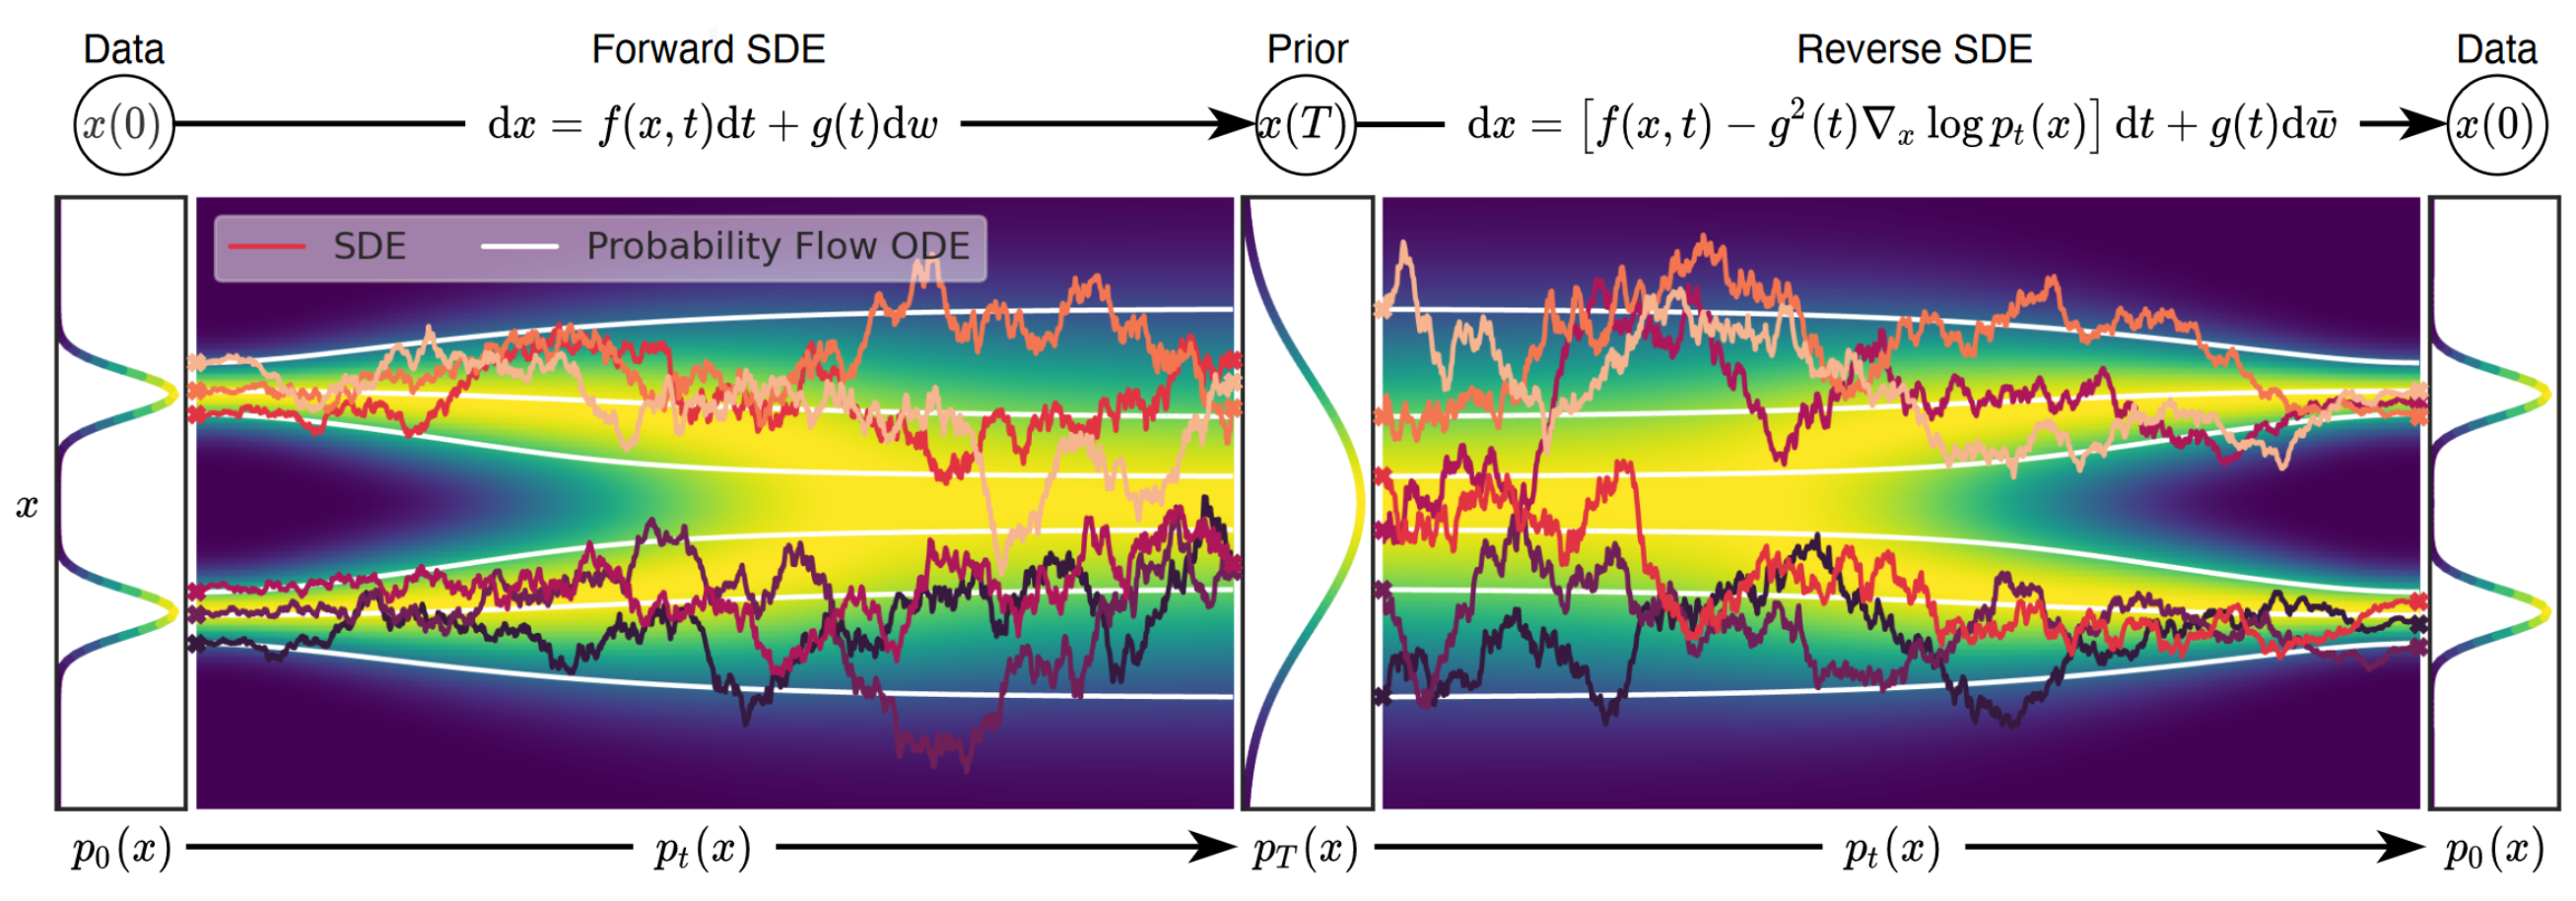
\includegraphics[width=1\columnwidth]{figures/DiffusionModels_SDEs.png}
    \caption{Summary of the score-based generative modeling through SDEs \citep{song2020score}}\label{fig:DM_SDEs}
\end{figure}

Knowledge of the scores at each time requires the estimation of the scores for an SDE which involves training a model to approximate the gradient of the log probability of data at various noise levels \citep{song2020score}. The training objective is given by:

\[
\theta^* = \arg\min_\theta \mathbb{E}_t \left\{ \lambda(t) \mathbb{E}_{x_0} \mathbb{E}_{x_t|x_0} \left\| s_\theta(x_t, t) - \nabla_{x_t} \log p_{0t}(x_t | x_0) \right\|_2^2 \right\}
\]

\citep{song2020score} The equation presents a method to find optimal model parameters \( \theta^* \) that minimize the expected discrepancy between the scores estimated by the model and the actual data transition scores over time, which are influenced by the noise \citep{song2020score}. The expectations are taken over time and modulated by a time-varying weighting function \( \lambda(t) \). ``With sufficient data and model capacity, score matching ensures that the optimal solution for the above equation, denoted by \(s_\theta*(x, t)\) equals \(\nabla_{x_(t)} \log p_{t}(x)\) for almost all \( x \) and \( t \)'' \citep{song2020score}. The score matching process matches the output of the score network with the true gradient of the log-likelihood over the course of the SDE, enabling the generation of realistic data samples from complex distributions \citep{yangdiffusionSummary}.
